\section{Bluetooth \textit{vs.} Wi-Fi Direct in Android Devices}
\label{sec:btvswifi}

In this section the data rates of both Bluetooth and Wi-Fi Direct will be analysed and compared. Since the data rates are technology specific, instead of conducting experiments that may not provide the most accurate results, a paper will be described, containing appropriate and accurate tests for these technologies' throughputs.

Bluetooth version 4.0 provides a theoretical, maximum throughput of \textit{24Mbps}, from \cite{bluetoothspec}, whereas Wi-Fi Direct provides a maximum throughput of \textit{250Mbps}, as stated in \cite{wfdrate}. To provide a precise measurement of both Bluetooth and Wi-Fi Direct's actual throughput in Android devices, the work developed by A. Mtibaa \textit{et al.} in \cite{throughputpaper} will be described. 

The devices used were two Google Nexus 5 smartphones running Android version 4.4.4, with Bluetooth 4.0. These devices were tested in three distinct environments: indoor line-of-sight, in an underground walkway \textit{350m} long and \textit{10m} wide. Indoor with obstacles, consisting of a set of offices separated by walls, \textit{4m} apart. Outdoor line-of-sight, in an outdoor walkway with \textit{582m} long and \textit{8m} wide.

Two sets of three experiments were conducted: one in each environment, using both communication technologies. In each experiment the throughput was measured by establishing a \gls{TCP} connection beetween client and server and sending \textit{5MB} files. The server then measured the total number of received bytes over \textit{2s} intervals, computing the throughput in that period.

In Figure \ref{fig:btthroughput} it is possible to see the measured devices' throughput, using Bluetooth, in the three described environments, as a function of the distance between devices.

Figure \ref{fig:btin} shows a plot of the throughput measurements in the indoor line-of-sight environment. It is possible to see that the maximum throughput achieved when both devices are in the same position, is \textit{2Mbps}. The throughput drops to almost half its initial value at a distance of \textit{20m}. At a distance of \textit{140m} the devices are not able to communicate.

Figure \ref{fig:btobs} shows a plot of the throughput measurements in the indoor with obstacles environment. The maximum throughput is \textit{0.9Mbps}, when the devices are in the same position. As the distance increases, the throughput decreases, in a linear fashion. At a distance of 5 offices (\textit{20m}), the devices can no longer communicate.

Figure \ref{fig:btout} shows a plot of the throughput measurements in the outdoor line-of-sight environment. A maximum throughput of \textit{0.6Mbps} is achieved in the initial position. The throughput drops to, around, \textit{0.2Mbps} at \textit{40m}, slightly decreasing until a distance of \textit{120m} separates the devices, preventing communication between them.

\begin{figure}[ht]
	\centering
	\subcaptionbox{Throughput in indoor line-of-sight.\label{fig:btin}}{
		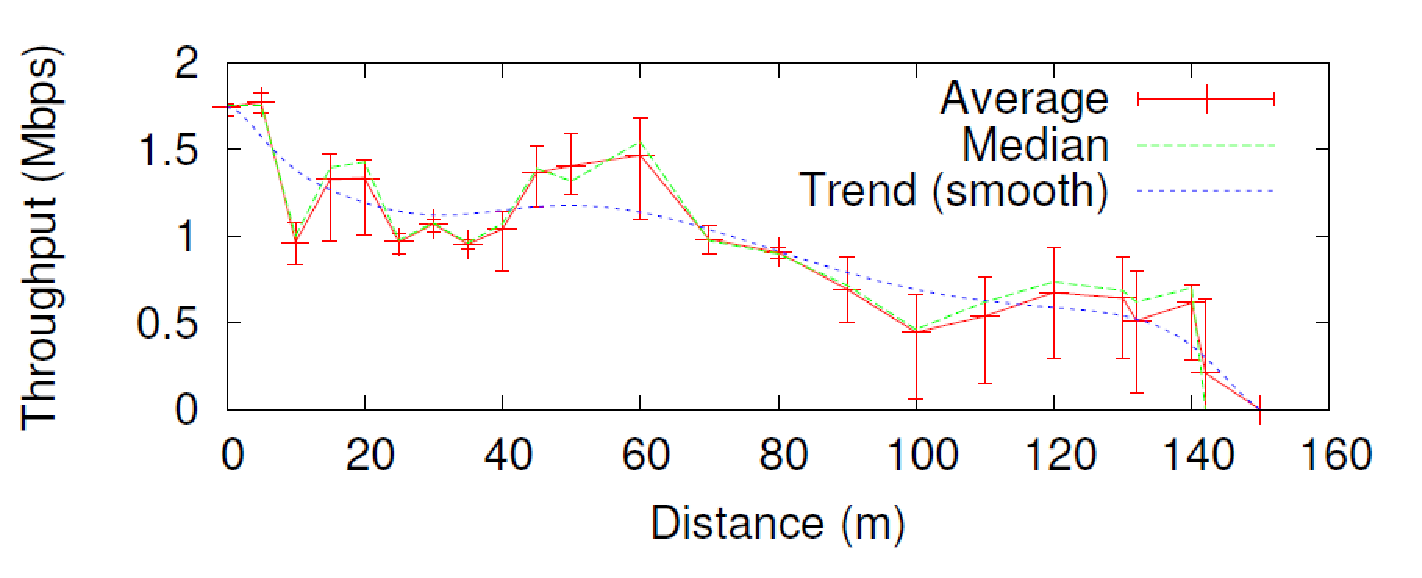
\includegraphics[width=0.7\textwidth]{images/btin.pdf}
	}\par\medskip
	\subcaptionbox{Throughput in indoor with obstacles.\label{fig:btobs}}{
		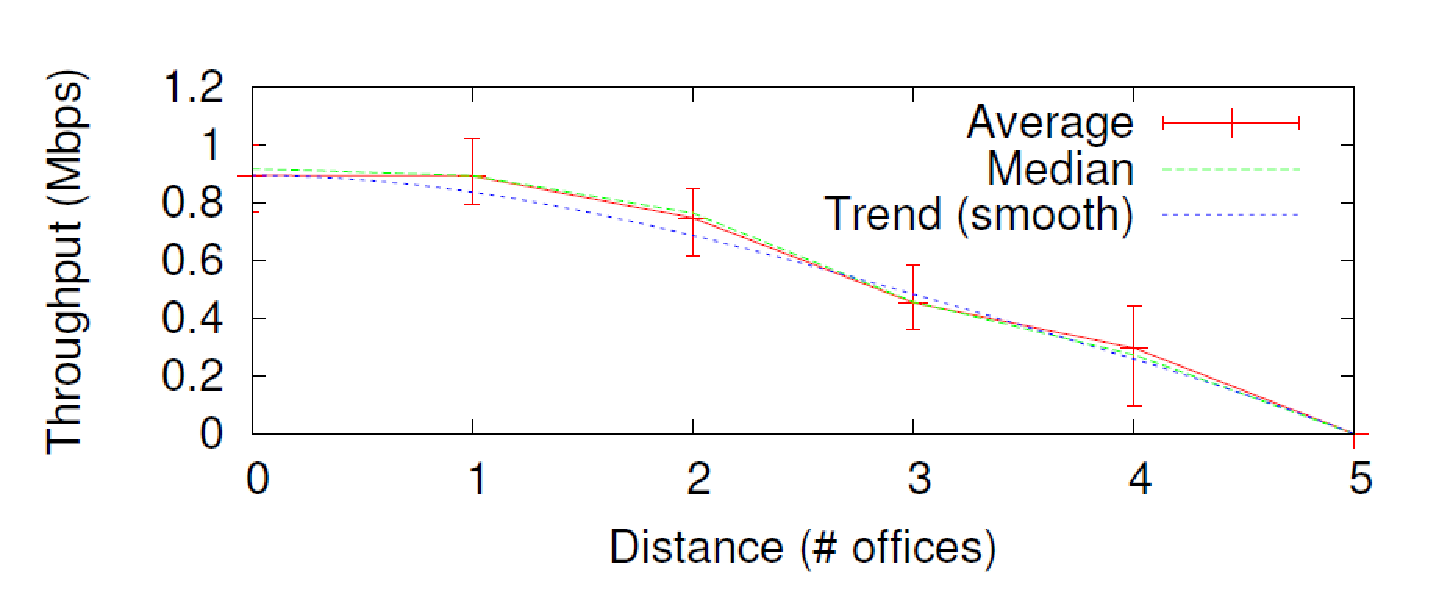
\includegraphics[width=0.7\textwidth]{images/btobs.pdf}
	}\par\medskip        
	\subcaptionbox{Throughput in outdoor line-of-sight.\label{fig:btout}}{
		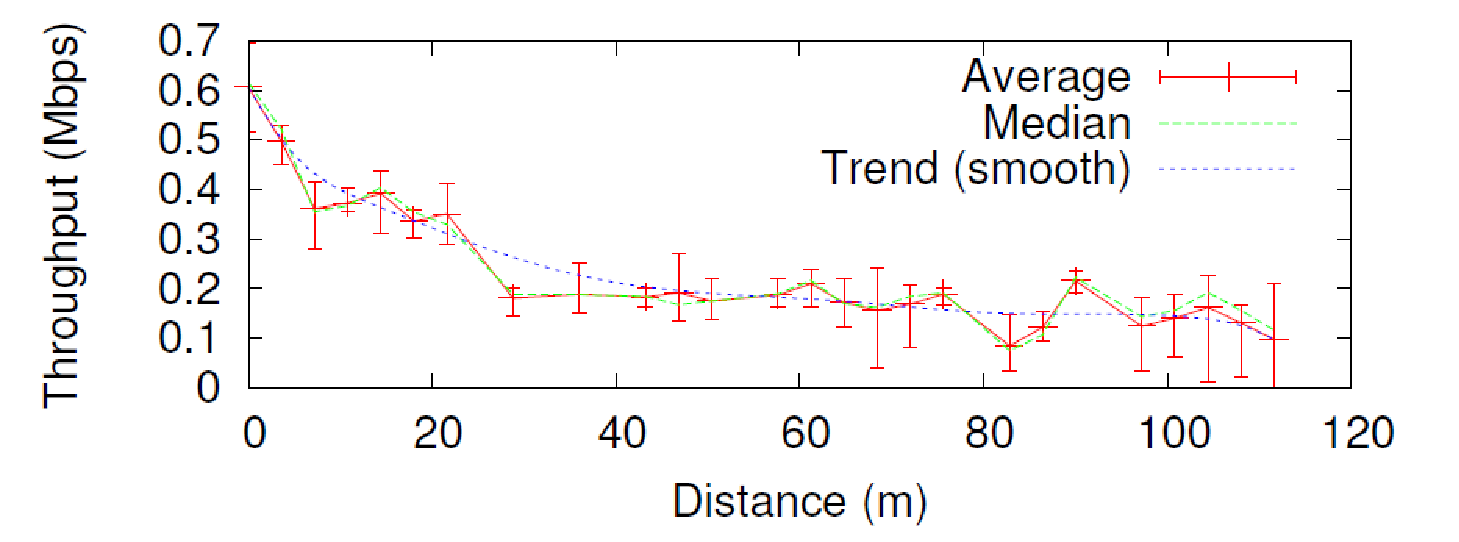
\includegraphics[width=0.7\textwidth]{images/btout.pdf}
	}
	\caption{Android Bluetooth single-hop throughput measurements in different environments (source \cite{throughputpaper}).}
	\label{fig:btthroughput}
\end{figure}

Overall, the devices using Bluetooth were able to communicate from \textit{20m} with obstacles, similarly to what was observed in \ref{subsec:ranges}, to \textit{150m} in the indoor line-of-sight environment. This disparity in the Bluetooth coverages comes from the phenomenon of signal reflections in the indoor environment, increasing the Bluetooth signal and consequently, its range. The throughput varied from \textit{0.6Mbps}, in the outdoor line-of-sight environment, to \textit{2.0Mbps}, in the indoor line-of-sight environment. This difference may be due to the channel interference, more prone to occur in the outdoor environment. 

Comparing the obtained measurements with the theoretical values, it can be said that (1) the throughput was significantly lower than what was stipulated in \cite{bluetoothspec} -- although, \gls{TCP} packets were used to measure the throughput, which may incur into further delays, as mentioned by the authors; (2) the communication ranges were much higher than the theoretical stipulation of \textit{10m} for Class 2 devices, which most smartphones are -- see \cite{bluetoothspec} -- however, for higher communication ranges, the throughput is much smaller, sometimes almost zero, as seen in Figure \ref{fig:btout}.

In Figure \ref{fig:wfthroughput}, it is possible to see the measured throughput of the devices, when communication via Wi-Fi. The authors state that, even though the showed results are obtained using Wi-Fi, the conclusions can be drawn to Wi-Fi Direct, as the results are redundant.

Figure \ref{fig:wfin} represents a plot of the measured throughput in the indoor line-of-sight environment. At a distance of \textit{0m}, the maximum throughput of \textit{40Mbps} is achieved. It then linearly decreases until a distance of \textit{125m}, where the throughput is almost null. At a distance of \textit{200m} the throughput is, roughly, \textit{1Kbps}.

Figure \ref{fig:wfobs} shows the measured throughput in the indoor with obstacles environment. At a distance of \textit{0m}, the measured throughput is \textit{30Mbps}. The indoor with obstacles environment presents a similar throughput decay as the one presented in Figure \ref{fig:wfin}. At a distance of 4 offices (\textit{100m}), the throughput measured less than \textit{5Mbps}.

In Figure \ref{fig:wfout}, the measured throughput in the outdoor line-of-sight environment is shown. At a distance of \textit{0m}, the throughput measures \textit{35Mbps}. However, at a distance of \textit{50m}, it measured less than \textit{5Mbps}. Despite what happened in the two previous environments, in the outdoor line-of-sight environment, the throughput decayed exponentially with the distance. At a distance of \textit{200m}, the throughput reaches \textit{0.8Mbps}, a much higher value than the one registered in the indoor line-of-sight environment.

\begin{figure}[ht]
	\centering
	\subcaptionbox{Throughput in indoor line-of-sight.\label{fig:wfin}}{
		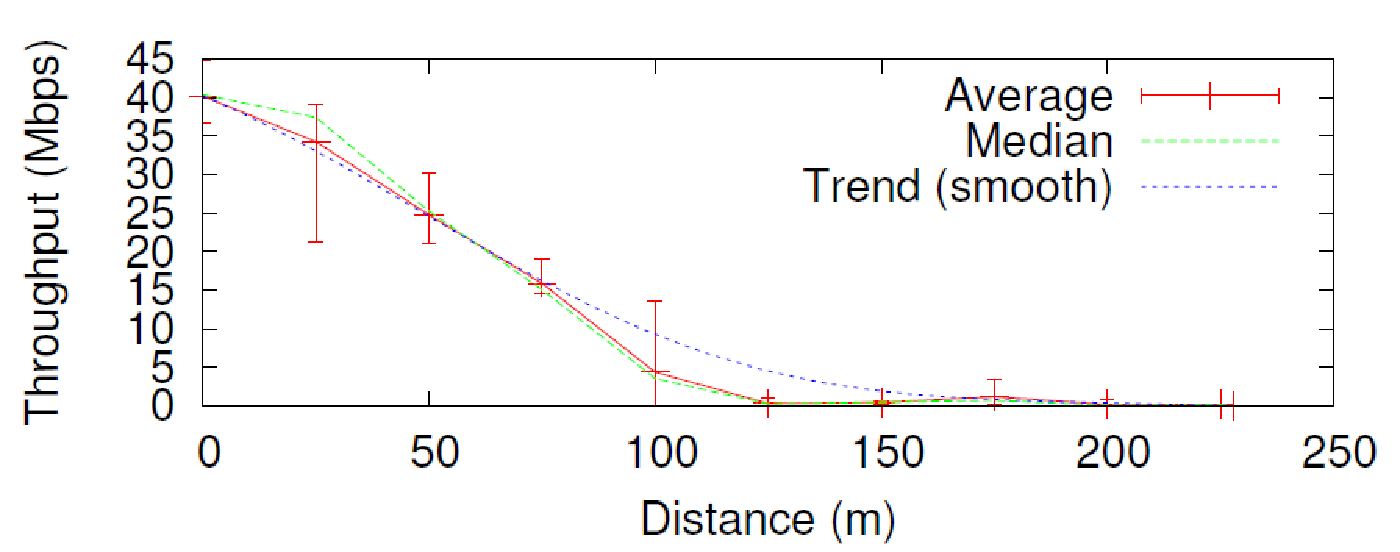
\includegraphics[width=0.7\textwidth]{images/wfin.pdf}
	}\par\medskip
	\subcaptionbox{Throughput in indoor with obstacles.\label{fig:wfobs}}{
		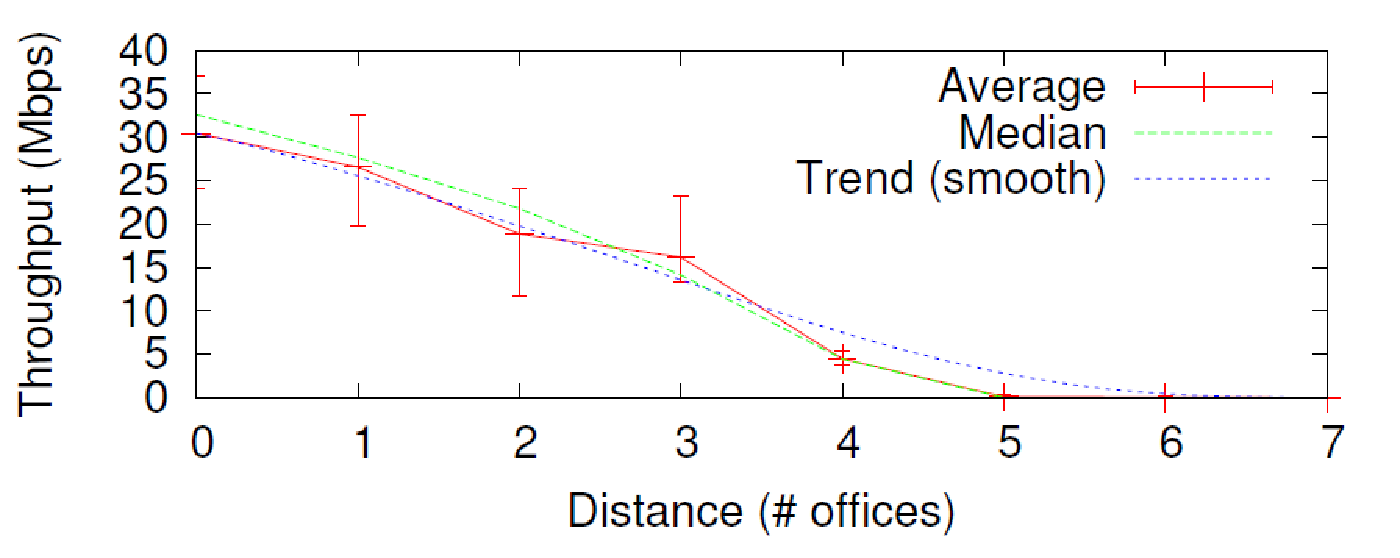
\includegraphics[width=0.7\textwidth]{images/wfobs.pdf}
	}\par\medskip        
	\subcaptionbox{Throughput in outdoor line-of-sight.\label{fig:wfout}}{
		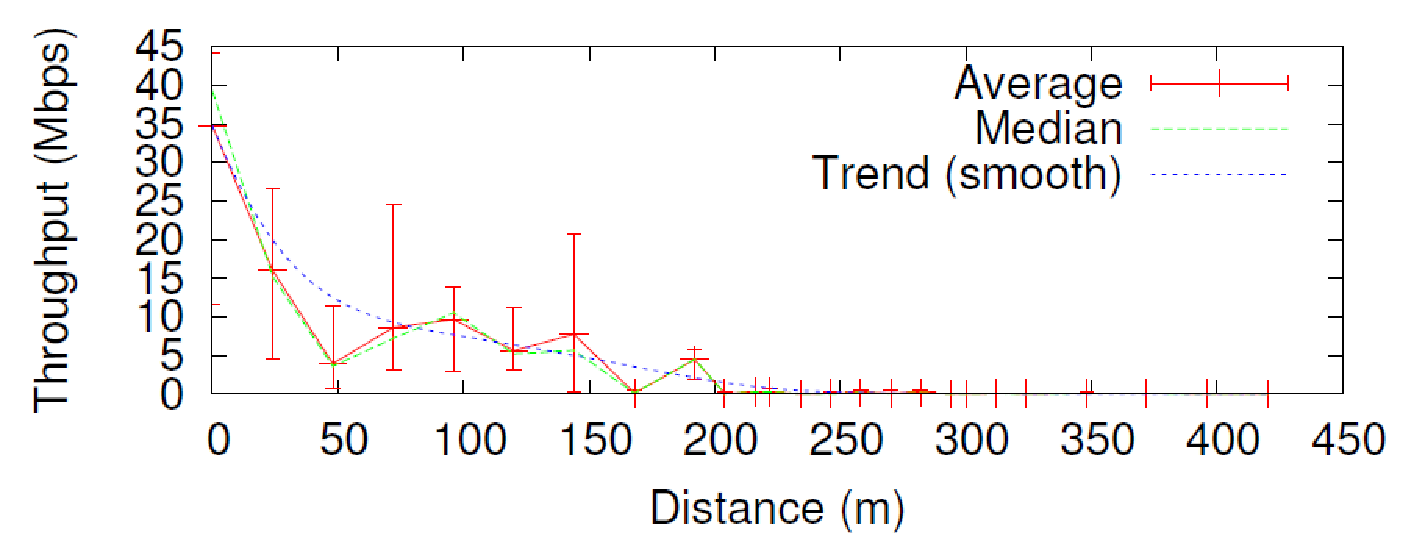
\includegraphics[width=0.7\textwidth]{images/wfout.pdf}
	}
	\caption{Android Wi-Fi single-hop throughput measurements in different environments (source \cite{throughputpaper}).}
	\label{fig:wfthroughput}
\end{figure}

After the brief analysis of the shown plots, it is possible to say that the indoor line-of-sight and indoor with obstacles environment present a similar throughput trend (in blue). In the outdoor line-of-sight environment, however, the throughput decays faster, in an exponential manner. This difference is due to the fact that propagation delay spreads are much smaller in indoor environments than outdoor environments. Having bigger delays, some reflections of the signal do not reach the server device during the \textit{2s} measured intervals, reducing the throughput.

However, at distances longer than \textit{200m}, outdoor environments show a much higher throughput than indoor environments. This is due to the fact that reflected and scattered signals are cancelled by signal attenuation, highly reducing the throughput and, as mentioned before, the reflection and scattering phenomena are more relevant in indoor environments.

It is also possible to state that, the throughput has never reached the theoretical value of \textit{250Mbps}. The maximum throughput measured was in the indoor line-of-sight environment with a value of \textit{40Mbps}, less than a fifth of the maximum theoretical value.

Further analysis of Bluetooth and Wi-Fi Direct's performance in Android devices will be shown in Section \ref{sec:btvswifitests}.